\section{Problem Setting}

\begin{frame}
	\begin{figure}[t]
		\centering
		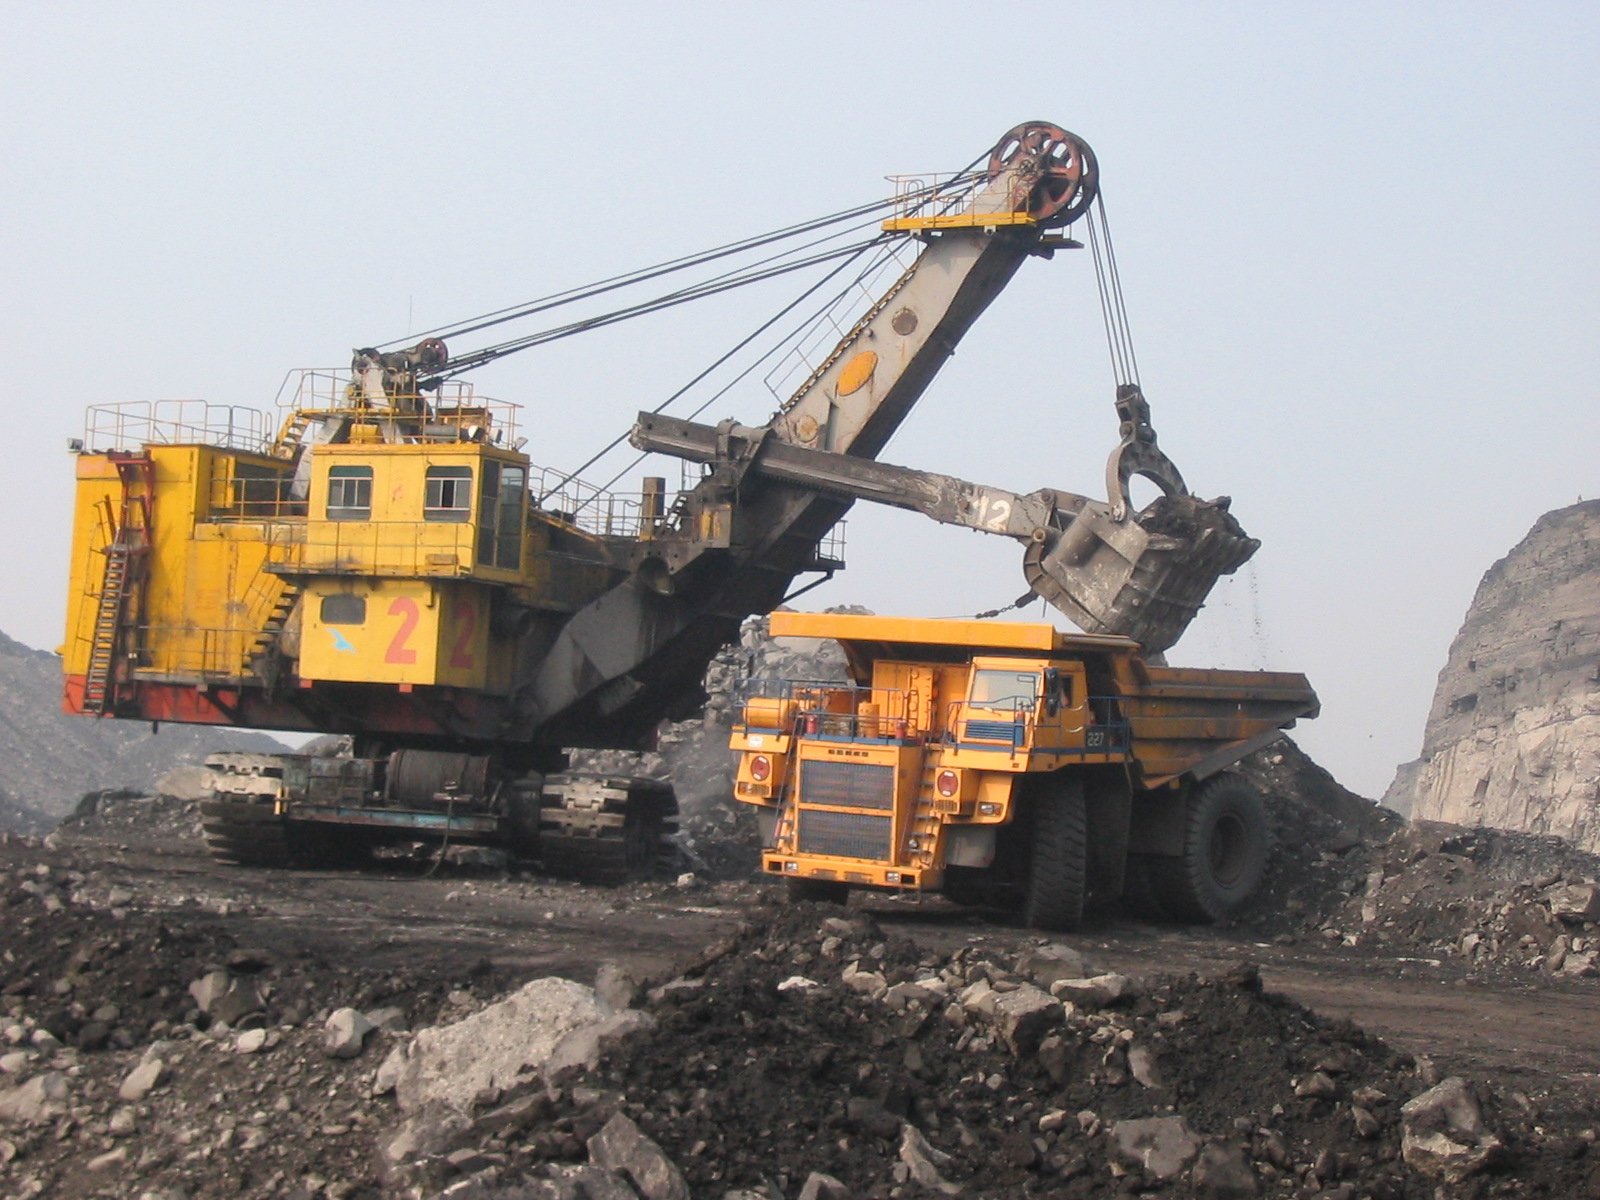
\includegraphics[width=.6\linewidth]{img/Excavator} \\
		\tiny{originally posted to Flickr by FAndrey at http://flickr.com/photos/43301444@N06/4141786255}
	\end{figure}

	\begin{itemize}
		\item{Goal: \textbf{optimization of model parameters}}
		\item{Models of technical system = physical properties + control properties}
	\end{itemize}
\end{frame}

\begin{frame}
	\frametitle{Problem Setting}
	\begin{figure}[bth]
		\centering
		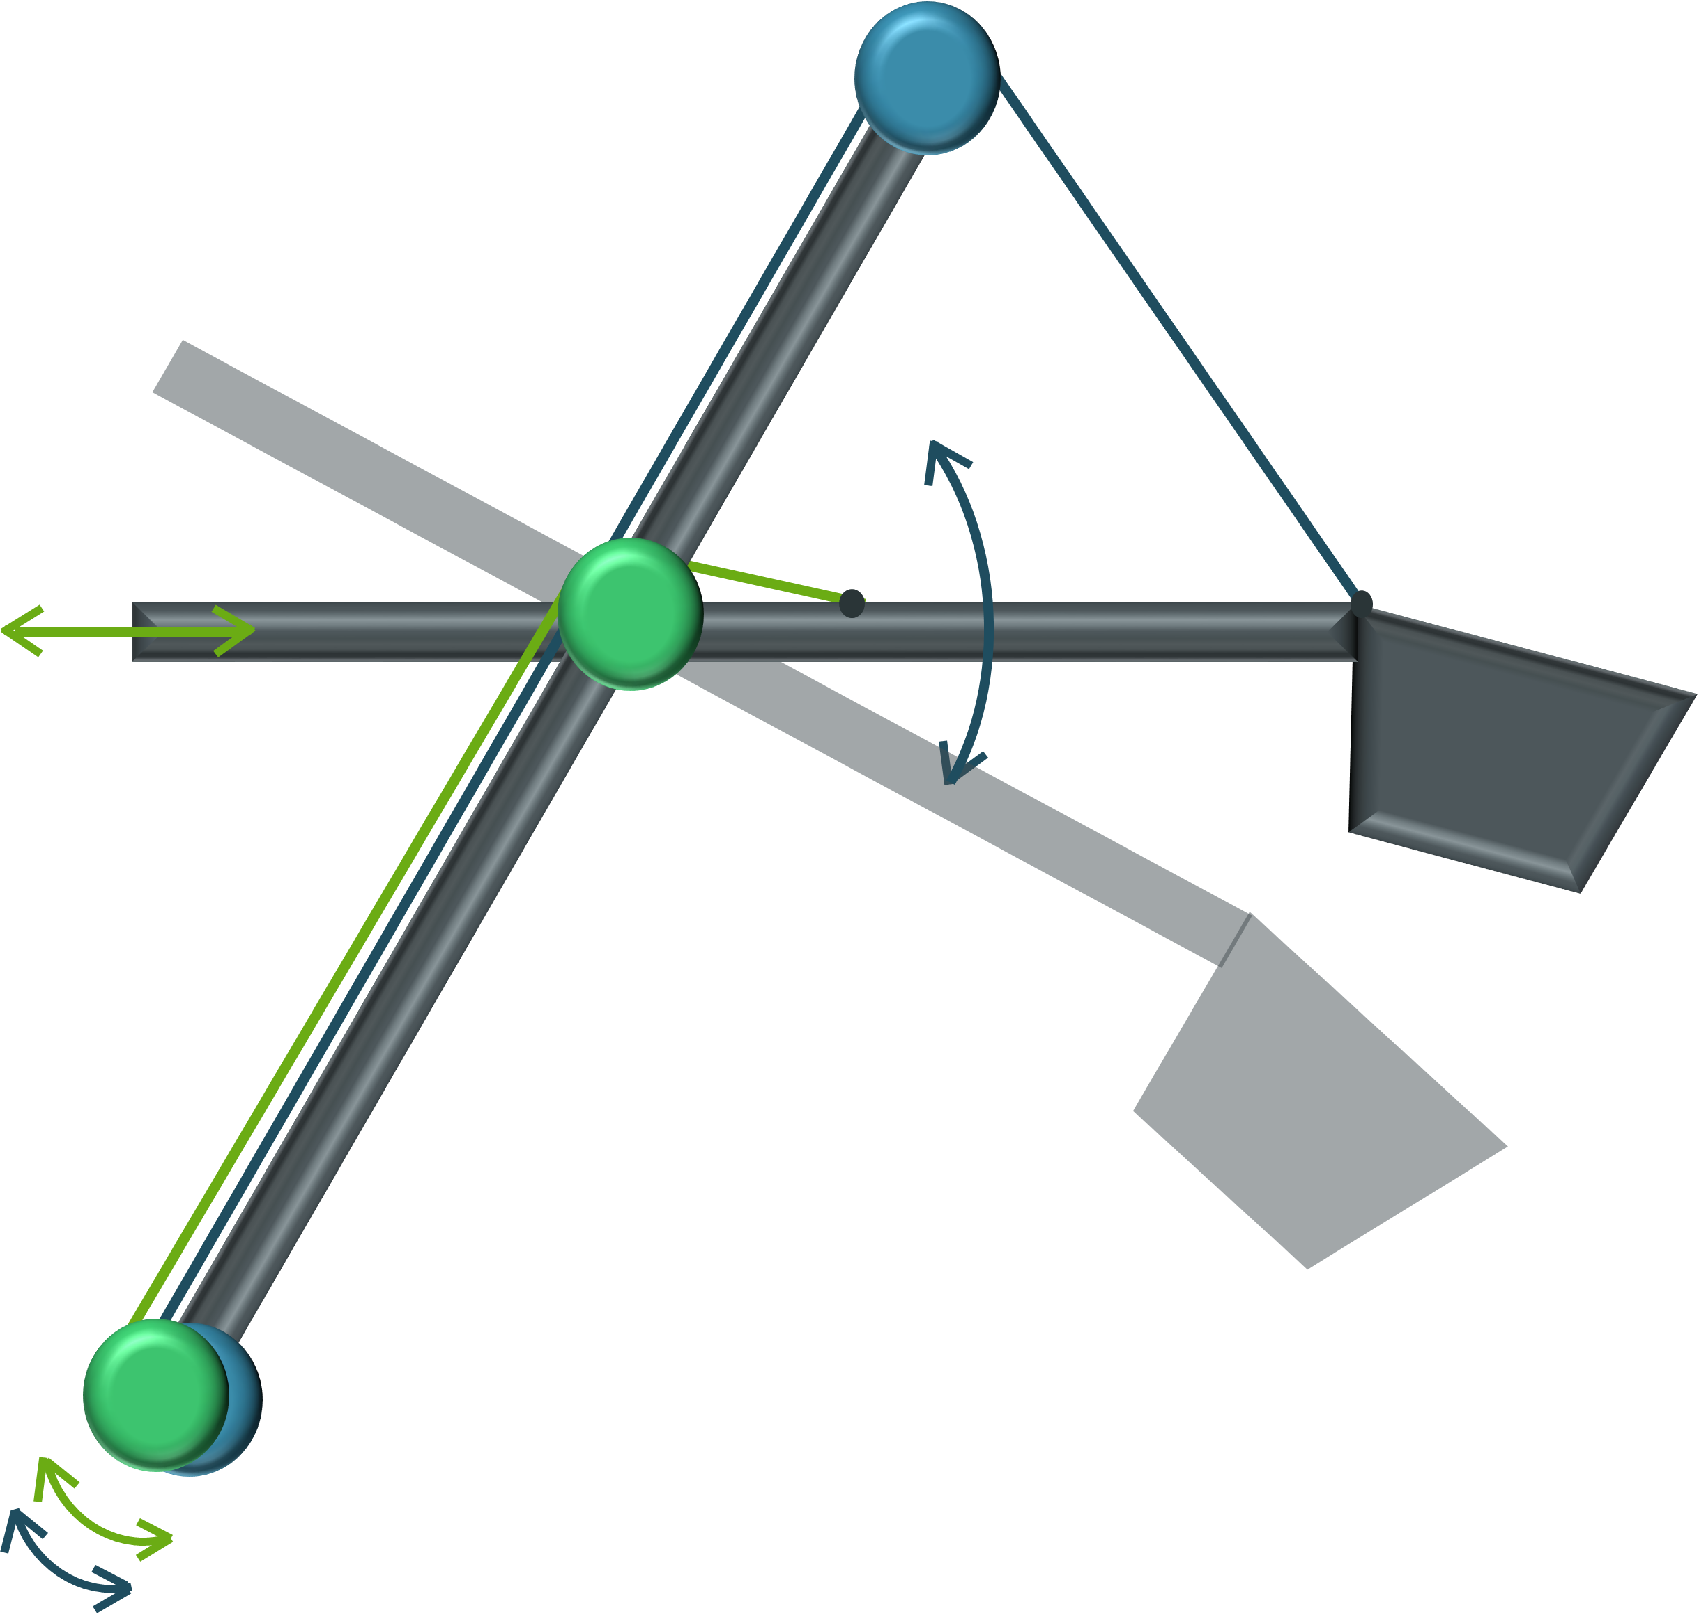
\includegraphics[width=.5\linewidth]{img/Problem_1}
	\end{figure}
\end{frame}

\begin{frame}
	\frametitle{Problem Setting}
	\begin{figure}[bth]
		\centering
		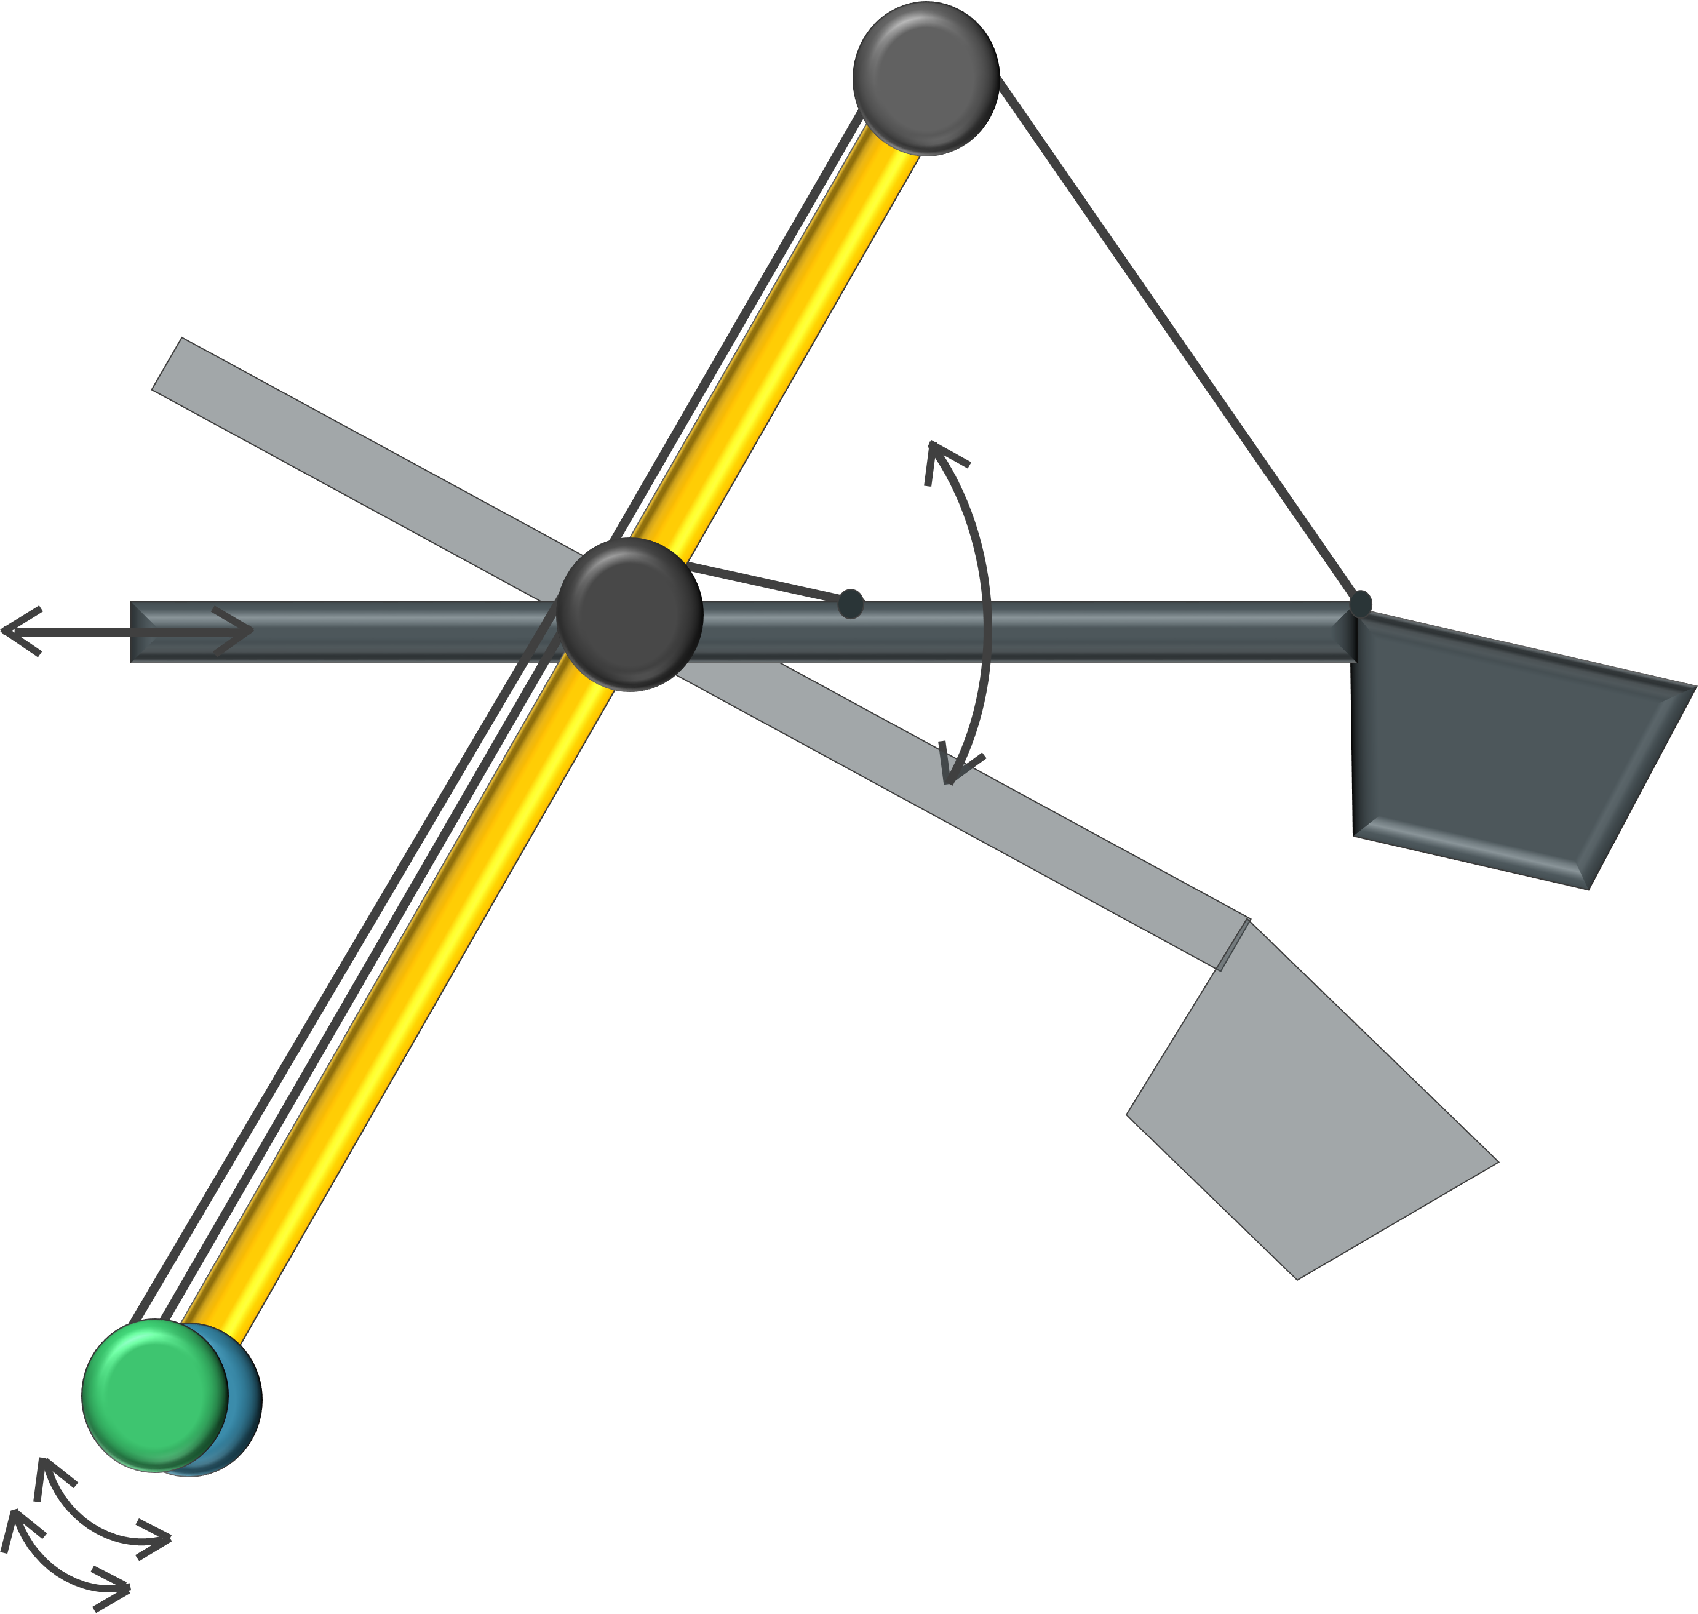
\includegraphics[width=.4\linewidth]{img/Problem_2}
	\end{figure}
	\begin{itemize}
		\item{arm element fixed to base}
		\item{cannot be moved w.r.t. the base}
	\end{itemize}
\end{frame}

\begin{frame}
	\frametitle{Problem Setting}
	\begin{figure}[bth]
		\centering
		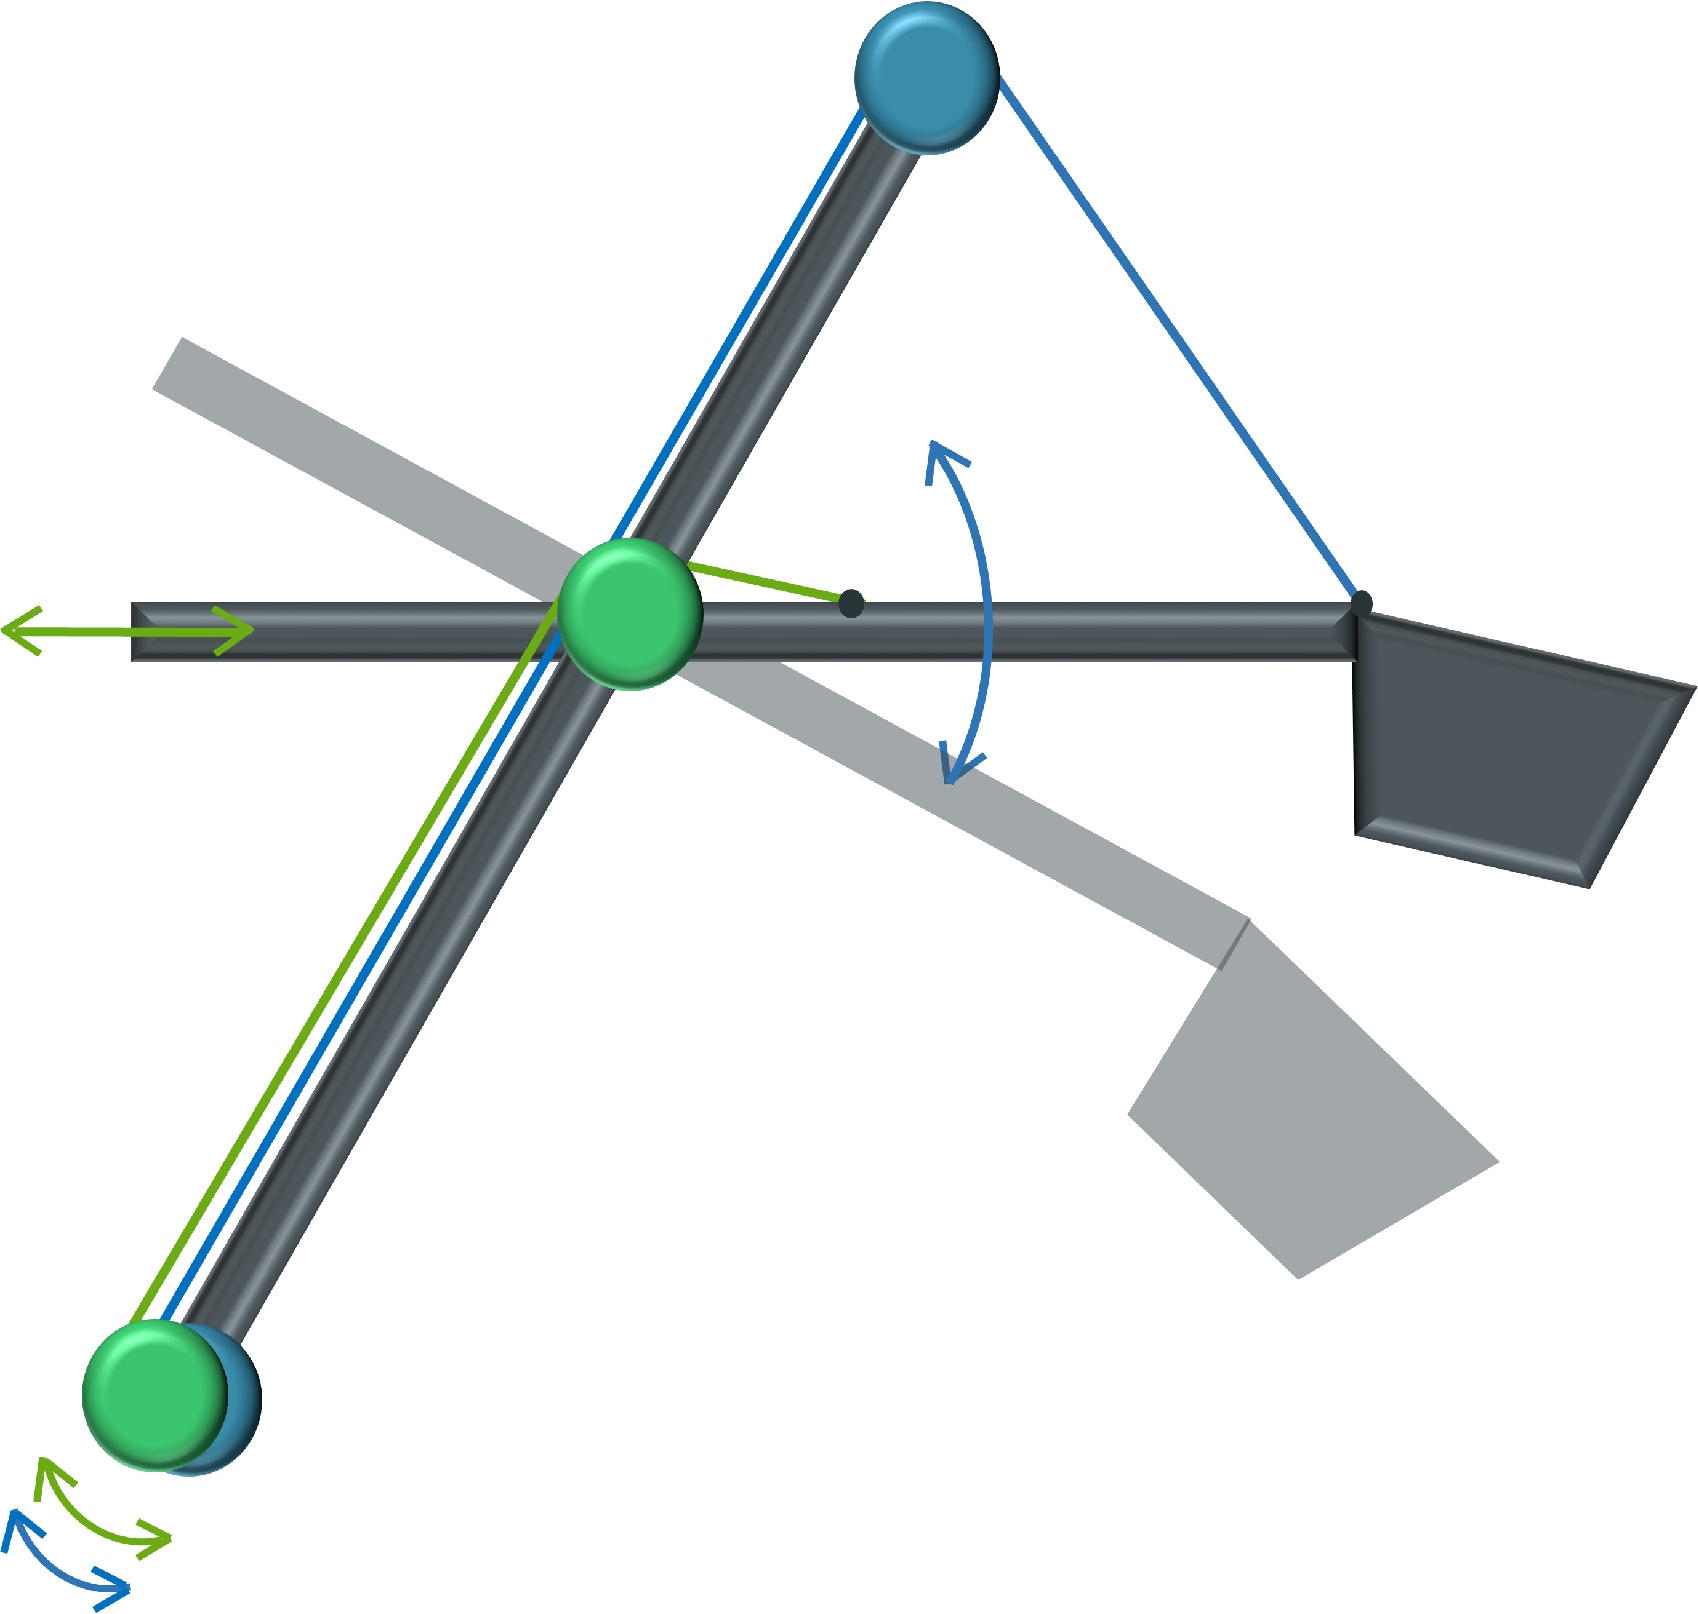
\includegraphics[width=.4\linewidth]{img/Problem_3}
	\end{figure}
	\centering
	\begin{itemize}
		\item{\makebox[1cm][l]{\textcolor[rgb]{0,0.69,0.32}{green}} shovel motion \textbf{back} and \textbf{forth}}
		\item{\makebox[1cm][l]{\textcolor[rgb]{0.18,0.46,0.71}{blue}} shovel motion \textbf{up} and \textbf{down}} \\
	\end{itemize}
\end{frame}

\begin{frame}[c]
	\frametitle{Main Problems}
	\onslide<1->
		\begin{enumerate}
			\item{Physical Modelling}
				\begin{itemize}
					\item{Modelling rope properties}
					\item{Determining information needed for calibration of model}
				\end{itemize}
			\vspace{0.5cm}
	\onslide<2>
			\item{Parameter Optimization}
				\begin{itemize}
					\item{Optimizing parameters for a complex, unknown model (black box)}
				\end{itemize}
		\end{enumerate}
\end{frame}

%\begin{frame}[c]
	%\frametitle{Physical Modelling}
	%\onslide<1->
		%Why?
		%\vspace{0.5cm}
		%\begin{columns}[t]
			%\column{.1\linewidth}
			%\column{.3\linewidth}
				%\centering
				%\fbox{\parbox{\textwidth}{Building an accurate model}}
			%\column{.2\linewidth}
				%\centering
				%$\Rightarrow$
			%\column{.3\linewidth}
				%\centering
				%\fbox{\parbox{\textwidth}{Good description of the effects of control and motion}}
			%\column{.1\linewidth}
		%\end{columns}
	%\onslide<2>
		%\vspace{1cm}
		%To consider:
		%\begin{itemize}
			%\item{Friction in cable reels}
			%\item{Deformation of ropes}
			%\item{etc.}
		%\end{itemize}
%\end{frame}

\begin{frame}[c]
	\frametitle{Physical Modelling}
	\onslide<1->
		Why?
		\begin{columns}
			\column{.4\textwidth}
				\centering
				\begin{tcolorbox}[width=\linewidth,colback={TUMblue}]
					Building an accurate model
				\end{tcolorbox}
			\column{.2\textwidth}
				\centering
				\Huge{$\Rightarrow$}
			\column{.4\textwidth}
				\centering
				\begin{tcolorbox}[width=\linewidth,colback={TUMblue1}]
					Good description of the effects of control and motion
				\end{tcolorbox}
		\end{columns}
	\vspace{0.5cm}
	\onslide<2>
		To consider:
		\begin{itemize}
			\item{Friction in cable reels}
			\item{Deformation of ropes}
			\item{etc.}
		\end{itemize}
\end{frame}

\begin{frame}
	\frametitle{Which color do we want to use?}
	\begin{tcolorbox}[width=\linewidth,colback={TUMblue}]
		TUMblue
	\end{tcolorbox}
	\begin{tcolorbox}[width=\linewidth,colback={TUMblue1}]
		TUMblue1
	\end{tcolorbox}
	\begin{tcolorbox}[width=\linewidth,colback={TUMblue2}]
		TUMblue2
	\end{tcolorbox}
	\begin{tcolorbox}[width=\linewidth,colback={TUMblue3}]
		TUMblue3
	\end{tcolorbox}
	\begin{tcolorbox}[width=\linewidth,colback={TUMblue4}]
		TUMblue4
	\end{tcolorbox}
	\begin{tcolorbox}[width=\linewidth,colback={TUMblue5}]
		TUMblue5
	\end{tcolorbox}
\end{frame}

%\begin{frame}[c]
	%\frametitle{Parameter Optimization}
	%\onslide<1->
		%What are parameters?
		%\begin{itemize}
			%\item{Friction coefficients}
			%\item{Mass}
			%\item{Inertia}
		%\end{itemize}
		%
		%\vspace{0.5cm}
	%
	%\onslide<2>
		%Why?
	%
		%\vspace{0.5cm}
	%
		%\begin{columns}
			%\column{.1\textwidth}
			%\column{.3\textwidth}
				%\centering
				%\fbox{\parbox{\textwidth}{Accurate and realistic parameters}}
			%\column{.2\textwidth}
				%\centering
				%$\Rightarrow$
			%\column{.3\textwidth}
				%\fbox{\parbox{\textwidth}{Better prediction and planning of motion}}
			%\column{.1\textwidth}
		%\end{columns}
%\end{frame}

\begin{frame}[c]
	\frametitle{Parameter Optimization}
	\onslide<1->
		What are parameters?
		\begin{itemize}
			\item{Friction coefficients}
			\item{Mass}
			\item{Inertia}
		\end{itemize}
	\vspace{0.5cm}
	\onslide<2>
		Why?
		\begin{columns}
			\column{.4\textwidth}
				\centering
				\begin{tcolorbox}[width=\textwidth,colback={TUMblue2}]
					Accurate and realistic parameters
				\end{tcolorbox}
			\column{.2\textwidth}
				\centering
				\Huge{$\Rightarrow$}
			\column{.4\textwidth}
				\begin{tcolorbox}[width=\textwidth,colback={TUMblue3}]
					Better prediction and planning of motion
				\end{tcolorbox}
		\end{columns}
\end{frame}